% !TEX root = ./main.tex
\section{Introduction}
Many highly contagious childhood diseases, such as measles, can be prevented by
vaccination. Therefore, it is worrisome that large outbreaks of such diseases 
have occurred in recent years, such as the measles
outbreaks in California in 2015 and in Minnesota in 2017---this is
despite high vaccination coverage in the US, e.g., $\sim 95\%$ for MMR, the measles vaccine. 
One of the reasons is the emergence of underimmunized geographical clusters, e.g., in California \cite{lieu2015geographic}
and Minnesota \cite{cadena:vacc-cluster}, often driven by misperceptions about 
side effects of vaccines \cite{atwell:pediatrics13}.  The typical response by public
health agencies is to monitor such clusters where immunization rates are falling, run active information campaigns, and engage community leaders. 

Cadena et al. \cite{cadena:vacc-cluster} use public school immunization data and identify six clusters in Minnesota,
which are statistically significant in terms of lower immunization rates, relative to the state wide level.
Implementing public health interventions in all these clusters is very expensive and time consuming for
public health agencies, which motivates the following problem: \textbf{\emph{which of these clusters (which are very different
in terms of size, immunization rates, and demographics) pose the most risk, and should be prioritized for response.}}
This is supported by Metcalf et al.~\cite{metcalf:epidemics15},
who state that \emph{``[t]here is also a need to understand under what conditions such clusters become at 
risk for epidemic spread, and the risk they pose to surrounding groups where vaccine coverage may be high.''} 
Since immunization rates are falling, it is useful to consider not only clusters in which these rates
are presently low, but also the clusters which would pose a risk if fewer people within them got vaccinated.
We develop a method to address these important public health policy questions.
Our contributions are summarized below.
\smallskip




\begin{figure}
\centering
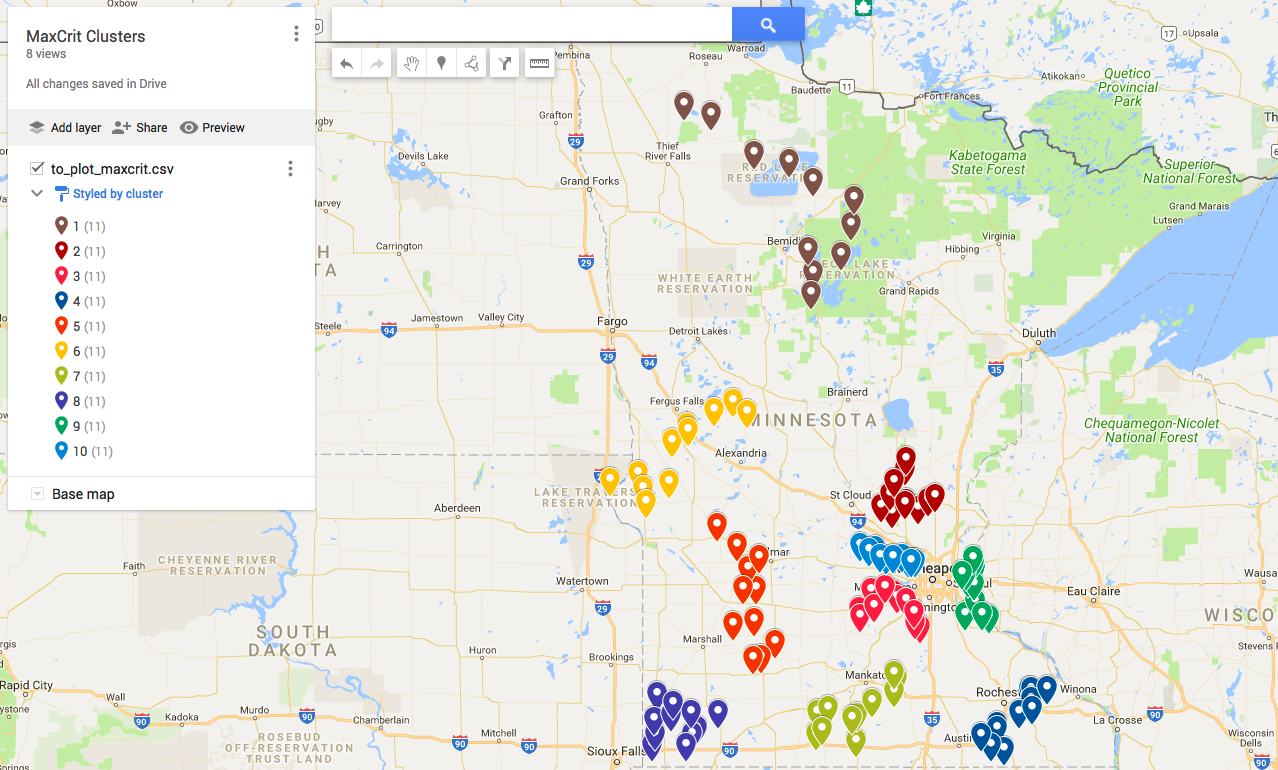
\includegraphics[width=.45\textwidth]{img/maxcrit_clusters.png}
\caption{Critical sets in Minnesota discovered using our methods. These are contiguous regions that lead to large measles outbreaks if not properly vaccinated.
\vspace*{-0.15in}
}
\label{fig:mn-criticalsets}
\end{figure}
%
%\begin{enumerate}
%\item 
\noindent
\textbf{1. Formalizing critical clusters.}
We formalize the notion of \emph{criticality} in a population represented as a social contact network $G=(V, E)$, with a spatial embedding $\HR$ (defined later). The criticality of a subset $S$ of the population is defined as the \emph{expected number of additional infections} that would occur if the immunization rate within $S$ is low. We are interested in clusters $S$ that (1) are contiguous in space, with respect to the spatial embedding network $\HR$ and (2) have the maximum criticality. We refer to this optimization task as the $\maxcrit{}$ problem. 

The spatial proximity is motivated by a public health response perspective, as in \cite{lieu2015geographic,atwell:pediatrics13,cadena:vacc-cluster}. Public health interventions involve intensive field work, and these interventions are most effective within a small region. This motivates the problem of finding a contiguous spatial cluster of bounded size with maximum criticality,
which are the kinds of clusters reported in \cite{cadena:vacc-cluster}.

%We formalize the notion of criticality in a social contact network $G=(V, E)$, which is associated with a spatial embedding, represented as a graph $\HR$ (defined formally later). The criticality of a subset $S$ is defined as the \emph{expected number of additional infections} that would occur if the immunization rate within $S$ is low. We are interested in clusters $S$ that 1) are contiguous in space and 2) have the maximum criticality---this is referred to as the \maxcrit{} problem. The spatial proximity is motivated by a public health response perspective, as in \cite{lieu2015geographic,atwell:pediatrics13}. Public health interventions involve intensive field work, which is another motivation for clusters corresponding to contiguous regions. Further, such response is most effective within a small region. This motivates the problem of finding a contiguous spatial cluster $S$ of bounded size with maximum criticality. Our contributions are as follows.


\noindent
\textbf{2. Rigorous algorithms for $\maxcrit{}$.}
The $\maxcrit{}$ problem is computationally very challenging. We show that \maxcrit{} is NP-hard and design algorithm \algomaxcrit{}, which has a worst case approximation guarantee of $\Omega(1/k^{(d-1)/(2d-1)})$, relative to the optimum, for clusters of size $k$. Here, $d$ is related to the complexity of the spatial embedding network $\HR$, and it is a constant in practice. 

We also show that the criticality function is submodular, which implies that $\maxcrit{}$ is equivalent to the classical Influence Maximization (\infmax) problem \cite{kempe:sigkdd03}, \emph{with an important constraint that the seed set is connected}. Due to this connectivity requirement, the standard greedy algorithms for \infmax{} yield poor results. %We also improve the running time significantly using a careful sampling technique.
A corollary of our results is an $\Omega(1/k^{(d-1)/(2d-1)})$ approximation for maximizing any non-negative monotone submodular function over the set of connected subgraphs of size $k$ in a graph with doubling dimension $d$. For any $d\geq0$, we have $1/k^{(d-1)/(2d-1)}\geq 1/\sqrt{k}$, so our result improves the previous best $\Omega(1/\sqrt{k})$-approximation for submodular maximization with connectivity constraints \cite{kuo2015maximizing}.

%Here, $d$ denotes the \emph{doubling dimension} of the associated spatial graph $\HR$ (defined later), and is a constant in practice, e.g., $2$ for a grid. We show that the \maxcrit{} objective is submodular, and this problem is equivalent to the classical Influence Maximization (\infmax) problem

%\item
\noindent
\textbf{3. Application.} 
We evaluate our algorithm on a detailed population and contact network model for the state of Minnesota.
The sets we discover have very high criticality compared to
heuristics commonly considered for public health interventions.
We achieve over 25\% higher criticality for the objective compared to all the baselines.
The critical clusters discovered using our algorithms (shown in Figure \ref{fig:mn-criticalsets})
have meaningful demographic properties
from a public health perspective: they typically involve people with lower than average
income and age (Section \ref{sec:experiments-cs}).
We also compute the criticalities of the clusters reported in \cite{cadena:vacc-cluster}.
Quite surprisingly, we find that: (1) the cluster with lowest vaccination rate among these is not the most critical, and
(2) the cluster computed using our algorithm has criticality more than 10 times that of any of the clusters
identified by \cite{cadena:vacc-cluster}.


Finally, because of the lack of public outbreak data, there is no easy way to validate our results, but we note that \emph{one of the clusters we found to be critical lies in the Minneapolis metropolitan area where a large measles outbreak occurred in 2017 \cite{hall:mmwr17}}.


\noindent
\textbf{Social impact.}
Our method for finding critical sets, applied to detailed population and contact network models (which are now standard approach in public health), provides an operational tool for public health agencies in prioritizing their limited surveillance and public outreach resources.
Our results imply that from a public health perspective, it is important to address not just the current undervaccinated clusters
identified in \cite{cadena:vacc-cluster}, but also make sure that the immunization rates in the critical clusters does not fall.






